\documentclass{article}
\usepackage{amsmath,amsthm,amssymb}
\usepackage {mathtext}
\usepackage{amsfonts} 
\usepackage[T1,T2A]{fontenc}
\usepackage[utf8]{inputenc}
\usepackage [english, russian] {babel}
\usepackage[babel=true]{microtype}
\usepackage{caption}
\usepackage{subcaption}
\captionsetup[table]{position=t,justification=raggedleft,slc=off}
\setlength{\abovecaptionskip}{0pt}
\usepackage {geometry}
\usepackage{graphicx}
\geometry{margin=1in}
\title{Лабораторная работа №1.2.5 \\ Исследование вынужденной регулярной прецессии гироскопа}
\author{Павел Рудачихин \\ Б04-507}
\date{27.11.2025}
\begin {document}
\maketitle{}
\section* {Аннотация} 

\hspace{4mm} \textbf{Цель работы:} исследовать вынужденную прецессию гироскопа; установить зависимость скорости вынужденной прецессии от величины момента сил, действующих на ось гироскопа; определить скорость вращения ротора гироскопа и сравнить её со скоростью, рассчитанной по скорости прецессии.

\textbf{В работе используются:} гироскоп в кардановом подвесе,секундомер, набор грузов, ротор гироскопа, металлический цилиндр, крутильный маятник, штангенциркуль, линейка, весы, осциллограф, генератор переменного напряжения. 

\textbf{Методы:} 1) определение  углового  коэффициента  наклона  зависимости двух величин; 2) измерение массы тел с помощью весов; 3) измерение времени с помощью секундомера.

\section* {Теоретические сведения}
\subsection* {Уравнения движения твёрдого тела}

\hspace{4mm} Твёрдое тело имеет 6 степеней свободы, поэтому для описания его движения необходимо и достаточно двух векторных уравнений: закона движения центра масс

\begin{equation}
	\frac{d\vec{P}}{dt} = \vec{F}
\end{equation}

и уравнения моментов

\begin{equation}
	\frac{d\vec{L}}{dt} = \vec{M}
\end{equation}

Здесь $\vec{P}$ - импульс тела, $\vec{F}$ - равнодействующая сила, $\vec{L}$ - момент импульса, $\vec{M}$ - момент равнодействующей силы.

\subsection* {Гироскоп}

\hspace{4mm} Момент импульса твёрдого тела в главных осях $x, y, z$ с базисными векторами $ \vec{i}, \vec{j}, \vec{k}$ равен

\begin{equation}
	\vec{L} = \vec{i} I_x \omega_x + \vec{j} I_y \omega_y + \vec{k} I_z \omega_z
\end{equation}

 Гироскопом называют быстро вращающееся тело, для которого с точностью до выбора осей выполнено $ I_x \omega_x \ll I_z \omega_z , \ I_y \omega_y \ll I_z \omega_z $.
 
 \begin{figure}[h!]
 	\centering
 	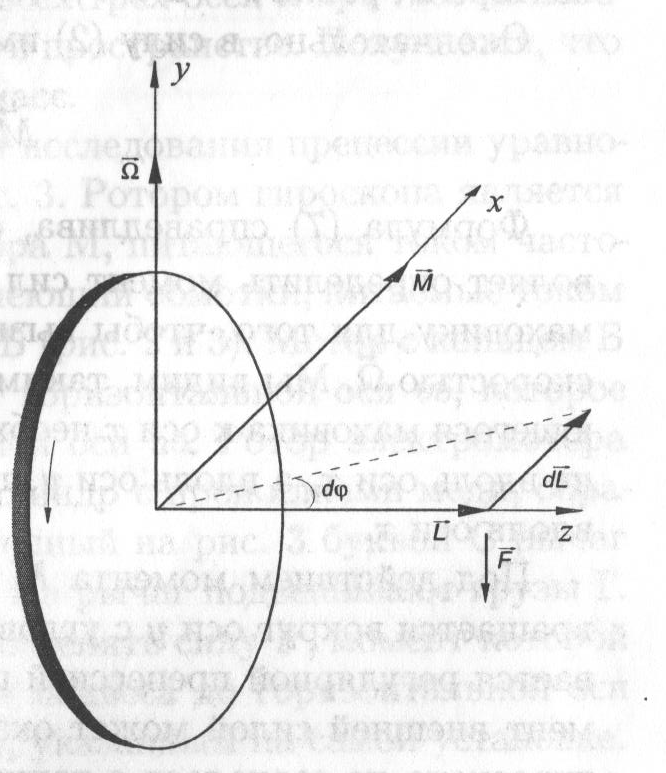
\includegraphics[width=0.5\linewidth]{1}
 	\caption{Вращение гироскопа: $L$ - момент импульса, $dL$ - его изменение за время $dt$ (поворот на угол $d\varphi$), $F$ - сила, приложенная к оси гироскопа, $M$ - её момент, $\Omega$ - угловая скорость прецессии.}
 	\label{fig:1}
 \end{figure}
 
 
 Рассмотрим вращение гироскопа вокруг оси $z$ с угловой скоростью $\omega$ (см. рис. 1). Можно показать, что, т.к. $L_\Omega \ll L_\omega$, вектор момента импульса будет вращаться в плоскости $xz$ со скоростью прецессии $\Omega$. Имеем основное уравнение теории гироскопа:
 
 \begin{equation}
 	\vec{M} = \vec{\Omega} \times \vec{L}
 \end{equation}

В данной работе сила $F$, приложенная к оси гироскопа, равна силе тяжести груза, подвешиваемого на расстоянии $l$ от оси вращения. Момент силы тяжести, действующей на гироскоп, можно не учитывать, так как гироскоп уравновешенный. Таким образом, угловая скорость прецессии равна

\begin{equation}
	\Omega = \frac{mgl}{I_z \omega}
\end{equation}

Используя (4), можно определить и момент сил трения в вертикальной оси гироскопа. Пусть за время $\tau$ ось опустилась на малый угол $\theta$. Тогда, пренебрегая изменением $L$ и считая $M_{тр}$ постоянным, положим угловую скорость прецессии, вызванной трением, неизменной и определим момент сил трения:

\begin{equation}
	M = \frac{\theta L}{\tau}
\end{equation}


\section*{Методика измерений}

\hspace{4mm} В работе измеряется время $t$, за которое гироскоп совершает $n$ оборотов вокруг вертикальной оси. Тогда, полагая $\Omega = 2\pi n/t$, выражаем угловую скорость вращения гироскопа:

\begin{equation}
	\omega = \frac{mglt}{2I \pi n}
\end{equation}  

Момент инерции гироскопа можно определить с помощью крутильного маятника. Известно, что период крутильных колебаний зависит от момента инерции тела $I$ и модуля кручения $f$:

\begin{equation}
	T = 2\pi \sqrt{\frac{I}{f}}
\end{equation} 

Измерив период колебаний $T_0$ тела c известным моментом инерции $I_0$, можно определить модуль кручения, затем, измерив период колебаний $T$ интересующего тела, определить его момент инерции:

\begin{equation}
	I = I_0 \frac{T^2}{T_0^2}
\end{equation}

В данной работе считается известным момент инерции сплошного цилиндра массой $M$ и радиуса $R$ относительно оси симметрии, параллельной образующей:
\begin{equation}
	I_0 = \frac{MR^2}{2}
\end{equation}

Есть способ определить $w$ иначе, что использовано для сверки результатов: статор гироскопа имеет две обмотки, одну из которых можно использовать для определения частоты вращения. Намагниченный ротор наводит в ней переменную ЭДС с этой же частотой. Подав на осциллограф в режиме X-Y напряжение с обмотки и с генератора, подобрав на нём частоту, можно получить устойчивую фигуру Лиссажу (эллипс) и определить частоту вращения ротора гироскопа.

\section*{Экспериментальная установка}

 \begin{figure}[h!]
	\centering
	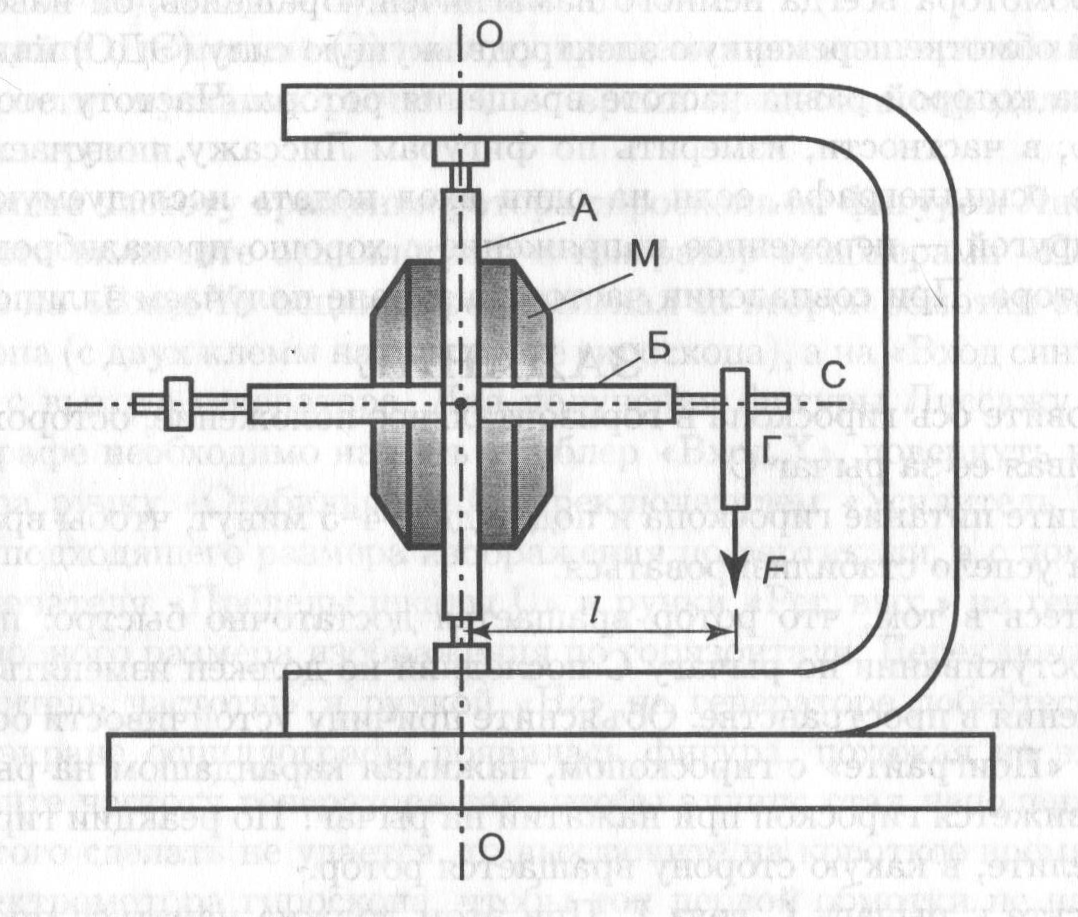
\includegraphics[width=0.6\linewidth]{2}
	\caption{Экспериментальная установка: М - электромотор, кольца А и Б образуют кардановый повес, С - рычаг,  Г - груз, OO - вертикаль, l - расстояние от неё до груза, F - сила тяжести груза.}
	\label{fig:2}
\end{figure}

 Схема установки приведена на рис. 2. Ротором гироскопа является ротор электромотора М. Статор мотора скреплён с кольцом Б. Кольцо Б может вращаться в кольце А. Рычаг С направлен по оси симметрии ротора. На него подвешивают грузы Г на расстоянии l от вертикальной оси ОО карданового подвеса.


\section*{Используемое оборудование}

\hspace{4mm} В данной работе для измерения массы использованы цифровые \textbf{весы}. Погрешность измерения массы определена как три в последнем разряде дисплея прибора: $\Delta_{\text{m}} = \pm 0,3$ г

Погрешность \textbf{линейки} составляет $\Delta_{\text{Л}} = \pm 0,5$ мм 

Погрешность \textbf{штангенциркуля} определена маркировкой производителя $\Delta_{\text{Ш}} = \pm 0,05$ мм 

Погрешность \textbf{секундомера} определена аналогично весам $\Delta_{\text{Ш}} = \pm 0,03$ с 

В работе использованы двухканальный \textbf{осциллограф} GOS-620 с полосой пропускания 20 МГц и \textbf{генератор-частотомер} АКИП-3408/3.

\section*{Результаты измерений и наблюдений}

\hspace{4mm} Длина рычага указана на установке: $l = (121 \pm 1)$ мм

Массы грузов и соответствующие им измеренные периоды прецессии приведены в таблице 1.
\begin{table}[h!]
	\centering
	\captionbox{Результаты измерений масс и периодов}{
	\begin{tabular}{|l|r|r|r|r|r|r|r|r|r|}
		\hline
		& 1        & 2        & 3        & 4        & 5     & 6     & 7        & 8        & 9 \\
		\hline
		$m$, г     & 56,1     & 59,8     & 75,5     & 92,8     & 111,2    & 141,1    & 214,1    & 266,6    & 334,2 \\
		\hline
		$T_1$, c     & 181,56   & 171,88   & 135,76   & 109,50   & 91,84    & 72,72    & 47,32    & 38,22    & 31,44 \\
		\hline
		$T_2$, c    & 181,74   & 172,18   & 135,62   & 109,94   & 92,18    & 72,82    & 47,79    & 38,03    & 31,84 \\
		\hline
		$T_3$, c      & 181,94   & 172,30   & 136,00   & 109,68   & 91,88    & 73,14    & 47,60    & 38,34    & 31,75 \\
		\hline
	\end{tabular}}

\end{table}%

В таблице 2 представлено время 15 колебаний ротора и цилиндра на крутильном маятнике.

\begin{table}[h!]
	\centering
	\captionbox{Время 15 крутильных колебаний}{
		\begin{tabular}{|c|c|}
			\hline
			$t_{ротора}$, c  & $t_{цилиндра}$, c  \\
			\hline
			48,10 & 59,93 \\
			\hline
			47,40  & 60,09  \\
			\hline
			47,53  & 60,19 \\
			\hline
	\end{tabular}}
\end{table}

Измерены масса цилиндра $M = (1616,0 \pm 0,3)$ г и диаметр цилиндра $2R = (78,00 \pm 0,05)$ мм

При частоте $\nu = 400$ Гц на осциллографе в режиме X-Y наблюдалась устойчивая фигура Лиссажу - эллипс (см. рис. 3).

Определено, что ось гироскопа опускается на $5^o$ за 382 с.

 \begin{figure}[h!]
	\centering
	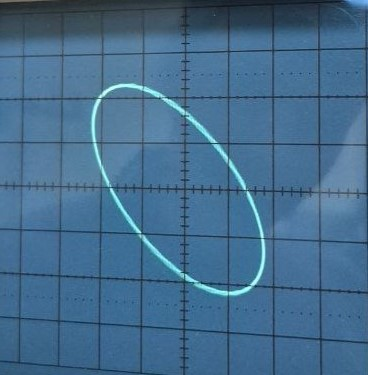
\includegraphics[width=0.6\linewidth]{3}
	\caption{Фигура Лиссажу на экране осциллографа в режиме X-Y}
	\label{fig:3}
\end{figure}


\section*{Обработка результатов}
\subsection*{Определение частоты вращения ротора гироскопа}

\subsection*{Определение момента импульса гироскопа}

%\begin{equation}
	%\sigma_{m_1 + m_2} = \sqrt{\sigma_{m_1}^{2} + %\sigma_{m_2}^{2}}
%\end{equation}

\hspace{4mm} Для каждого груза определим следующие величины.

Момент силы тяжести и его относительную погрешность:

\begin{equation}
	M = mgl \ \ \ \
	\varepsilon_M = \sqrt{\varepsilon_l^2 + \varepsilon_m^2}
\end{equation}

Средний период прецессии, его случайную и полную погрешности:

\begin{equation}
	T = \frac{1}{3} \sum_{i=1}^{3} T_i \ \ \ \
	\sigma_{сл} = \sqrt{\frac{1}{3} \sum_{i=1}^{3} (T_i - T)^2} \ \ \ \
	\sigma_{T} = \sqrt{\sigma_{сл}^2 + \sigma_{сист}^2}
\end{equation}

Угловую скорость, её относительную и абсолютную погрешности:

\begin{equation}
	\Omega = \frac{2\pi}{T} \ \ \ \
	\varepsilon_{\Omega} = \varepsilon_T = \frac{\sigma_{T}}{T} \ \ \ \
	\sigma_{\Omega} = \varepsilon_{\Omega} \Omega
\end{equation}

Построим график зависимости $\Omega = \Omega(M)$. По методу наименьших квадратов проводим лучшую прямую (см. рис. 4).

 \begin{figure}[h!]
	\centering
	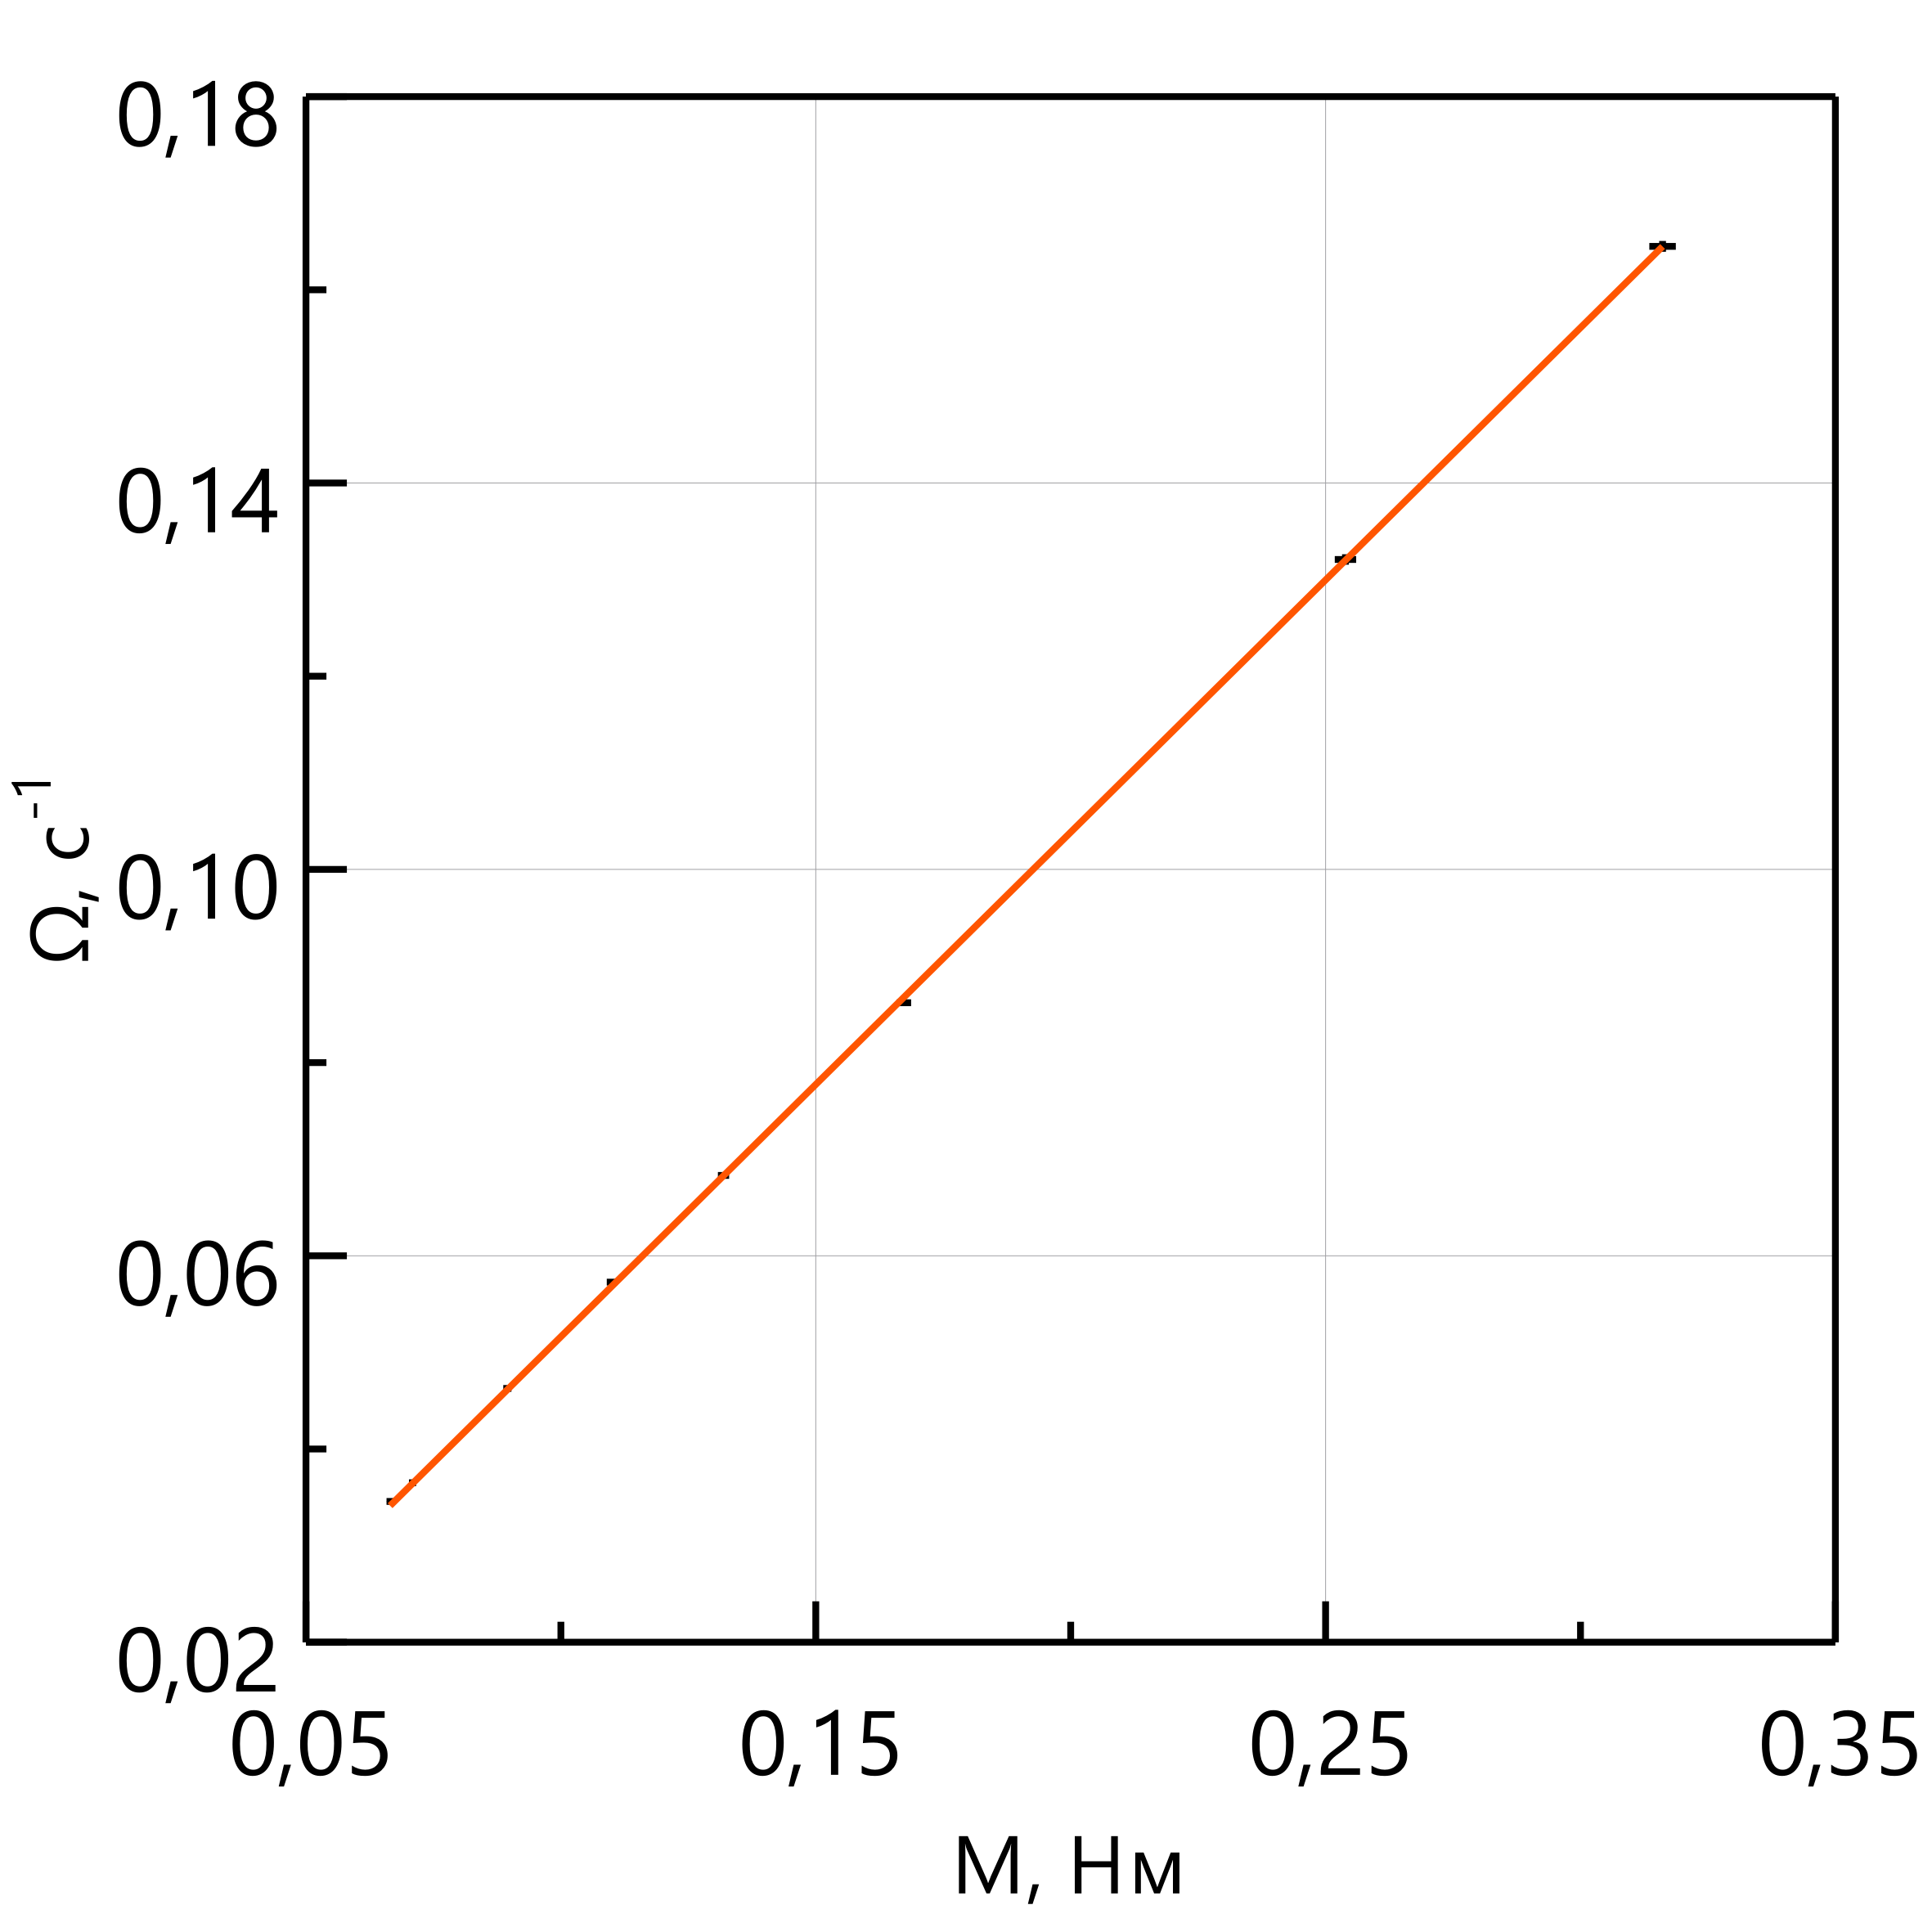
\includegraphics[width=0.6\linewidth]{4}
	\caption{График зависимости $\Omega = \Omega(M)$}
	\label{fig:4}
\end{figure}

 Получаем значения углового коэффициента $b$ и свободного члена $a$:

\begin{equation}
	b = (0,492 \pm 0,009)\ {(Нмс)^{-1}} \ \ \ 
	a = (0,002 \pm 0,003) \ {c^{-1}}
\end{equation}

Угловой коэффициент прямой - величина, обратная моменту импульса. Имеем:

\begin{equation}
	L = (2,03 \pm 0,04) {\frac{кг \cdot м^2}{c} }
\end{equation}


\subsection*{Определение момента инерции гироскопа}

\hspace{4mm} Аналогично периоду прецессии вычислим средний период крутильных колебаний ротора $T$ и цилиндра $T_0$ и их погрешности. Имеем:

\begin{equation}
	T = (3,18 \pm 0,02) \ c \ \ \ T_0 = (4,005 \pm 0,008) \ c
\end{equation}

Определим момент инерции цилиндра по формуле (10) и его относительную погрешность:

\begin{equation}
	I_0 = \frac{M R^2}{2} = \frac{1,616 \cdot 0,039^2}{2} \approx 0,0012289 \ (кг \cdot м^2)
\end{equation}

\begin{equation}
	\varepsilon_{I_0} =\sqrt{ \varepsilon_M^2 + 4 \varepsilon_R^2 }
\end{equation}

\begin{equation}
	I_0 = (1228,9 \pm 1,6) \cdot 10^{-6} \ кг \cdot м^2
\end{equation}

Вычислим момент инерции гироскопа по формуле (9). 

\begin{equation}
	I = I_0 \frac{T^2}{T_0^2} = 774,2 \cdot 10^{-6} \ кг \cdot м^2
\end{equation}

Определим его относительную погрешность:

\begin{equation}
	\varepsilon_{I} =\sqrt{ \varepsilon_{I_0}^2 + 4 \varepsilon_T^2 + 4 \varepsilon_{T_0}^2}
\end{equation}

Имеем 

\begin{equation}
	I =  (770 \pm 10) \cdot 10^{-6} \ кг \cdot м^2
\end{equation}

\subsection*{Определение частоты вращения ротора гироскопа}

Определим частоту вращения ротора гироскопа

\begin{equation}
	\nu = \frac{\omega}{2 \pi} = \frac{L}{2 \pi I} \approx 419 \ Гц
\end{equation}

и её относительную погрешность

\begin{equation}
	\varepsilon_{\nu} = \sqrt{ \varepsilon_{I}^2 +  \varepsilon_L^2 } \approx 2,3 \%
\end{equation}

\begin{equation}
	\boxed{\nu =  (419 \pm 9)\ Гц}
\end{equation}







Все вычисления произведены с помощью ПО Microsoft Excel. Построение графиков выполнено в программе LabPlot. 

\subsection*{Определение частоты вращения ротора гироскопа с получением фигуры Лиссажу}

Частота на генераторе установлена с точностью до 0,01 Гц. Поэтому результат измерения следующий

\begin{equation}
	\boxed{\nu =  (400,02 \pm 0,01)\ Гц}
\end{equation}

\subsection*{Определение момента сил трения}

По формуле (6) определим момент сил трения

\begin{equation}
	M = \frac{5}{180} \cdot \pi \frac{2,03}{382} \approx 0,0004 \ (Н \cdot м)
\end{equation}

Угол определён по метке на кольце карданового подвеса. Точность этой метки, к сожалению, не известна. Но нам достаточно показать, что момент сил трения много меньше момента силы тяжести. Минимальный момент силы тяжести составил 0,07 $Н \cdot м$, что на два порядка больше момента сил трения.

\section*{Анализ результатов}

\hspace{4mm} Полученные значения частот близки и различаются на 5\%. Относительная погрешность по прецессионному методу больше 2\%, а по методу получения фигуры Лиссажу составляет тысячные доли процента. Конечно, последний способ гораздо точнее. 

Все инструментальные погрешности малы, и основной вклад в итоговый результат вносит случайная погрешность измерения периодов. Она, например, для периода крутильных колебаний ротора гироскопа в десять раз больше систематической (0,3 с и 0,03 с соответственно). Действительно, работа с секундомером требует от экспериментатора высокой скорости реакции, которая не может быть измерена. Избавиться от этой проблемы можно с использованием датчиков, например, оптопары.

\section*{Заключение}

\hspace{4mm} Цели работы достигнуты: измерена частота вращения ротора гироскопа двумя методами; проверено, что влияние трения мало; получена линейная зависимость между угловой скоростью прецессии и моментом силы тяжести, что подтверждает основное уравнение теории гироскопа. Результат работы близок к ожидаемому. Определены основные источники погрешностей.

\end {document}